  \section{Accessibilit�}
Tutte le scelte progettuali sono state prese in base al tema dell'accesibilit�, seguendo le linee guida del W3C.\vspace{-0.3cm}
\subsection{Colori}
Si � evitato di utilizzare combinazioni di colori che potessero creare problemi di accessibilit�, usabilit� e comprensione del contenuto a persone affette da daltonismo. Si riportano di seguito degli screenshot di varie simulazioni di daltonismo della pagina Attivit�. Inoltre � stato mantenuto un contrasto pari a 7:1 tra il colore di sfondo e il colore dei testi.
\begin{figure}[h]
	\centering
	\subfloat[][\emph{Immagine Originale}]
	{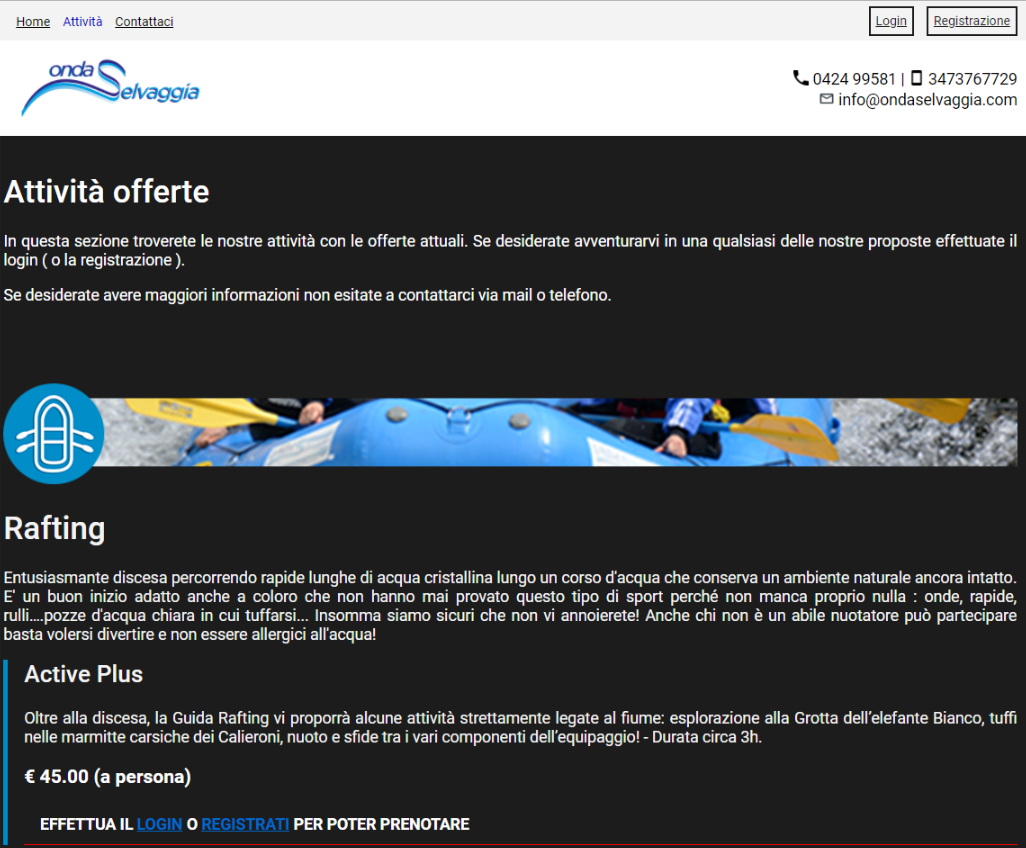
\includegraphics[scale=0.25]{images/normal_color.png}} \quad
	\subfloat[][\emph{Deutenatropia}]
	{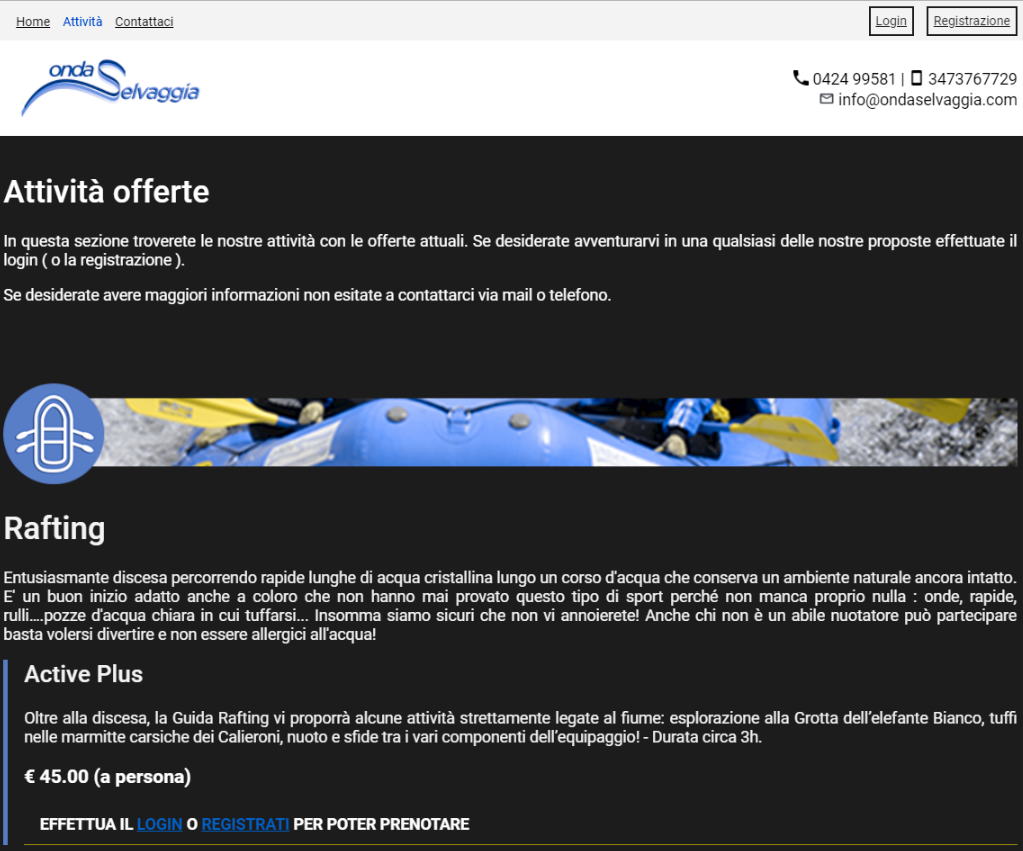
\includegraphics[scale=0.25]{images/deut.png}} \\
\end{figure}
\begin{figure}[h]
	\subfloat[][\emph{Protanopia}]
	{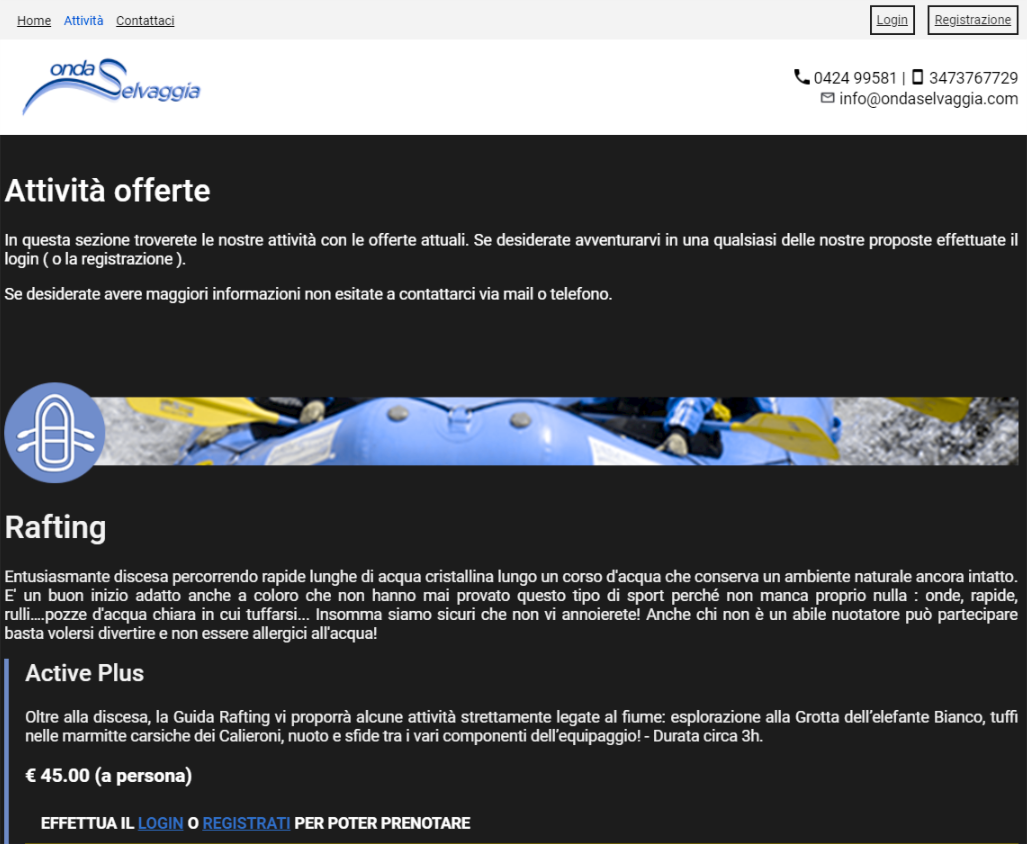
\includegraphics[scale=0.25]{images/tren.png}} \quad
	\subfloat[][\emph{Tritanopia}]
	{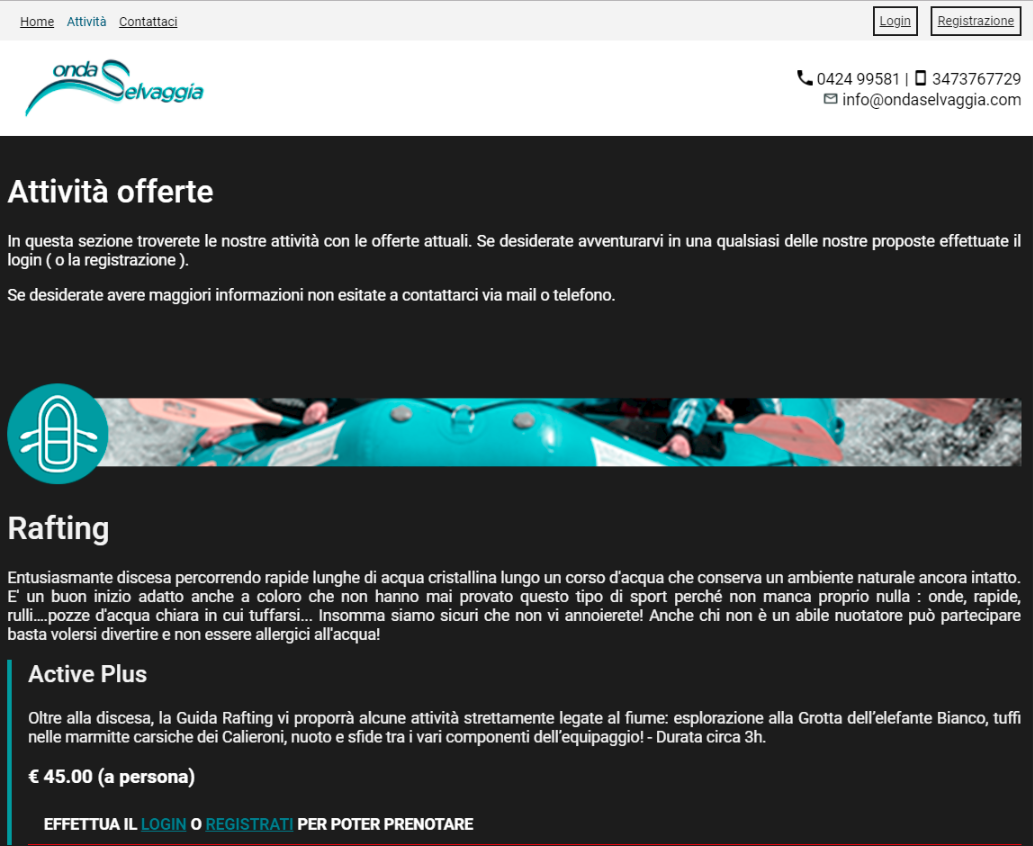
\includegraphics[scale=0.25]{images/tritano.png}} \\
	\caption{Simulazione di daltonismo}
\end{figure} \\

\newpage
\noindent
Per migliorare il contrasto il colore dei link � stato modificato rendendo comunque riconoscibili i link visitati e non.

\subsection{Tag}
Per quanto concerne i tag che migliorano l'accessibilit�:
\begin{itemize}
 	\item Sono stati utilizzati i tag \texttt{alt} per le immagini seguendo le linee guida del W3C.
 	\item Le parole in lingua inglese sono state racchiuse in un tag \texttt{<span lang="en"> </span>} cos� da poter garantire una lettura corretta da parte degli screen reader.
 	\item Sono stati utilizzati i tag \texttt{tabindex} in modo da permettere la navigazione corretta del sito attraverso il tasto TAB. Inoltre, poich� l'intestazione del sito si ripete per ogni pagina, � stato introdotta una voce del men� non visibile \texttt{Salta intestazione} che permette agli utenti che utilizzano uno screen reader di saltare la lettura dell'intestazione e passare direttamente al contenuto.
 	\item \'{E} stato utilizzato il tag \texttt{scope} dove necessario seguendo i dettami del W3C. Inoltre � stato evitato l'utilizzo di tabelle per realizzare il layout del sito.
 	\item Per rendere accessibili i form, sono stati utilizzati i tag \texttt{label, fieldset e title}, assieme ad una gestione degli errori che comprende  controlli di validit� dell'input.
\end{itemize}
\hypertarget{aria}{\subsubsection{Tag WAI-ARIA}}
Sono stati utilizzati dei tag introdotti dalle specifiche WAI-ARIA che permettono di migliorare l'accessibilit� per gli utenti che utilizzano uno screen reader. 
\paragraph{div di errore per i form}\mbox{}\\
Per segnalare all'utente degli errori di input nei vari form � stato creato un 
\texttt{div} che ha i seguenti attributi:
\begin{itemize}
	\item \texttt{aria-live="assertive"} Le tecnologie assistive (AT), come uno screen reader, notificano immediatamente all'utente la regione dichiarata \texttt{assertive}, in questo caso il \texttt{div} di errore verr� notificato e verranno letti gli errori, permettendo all'utente di correggere l'input.  
	\item \texttt{aria-atomic="true"} Indica allo screen reader di leggere interamente la regione di errore e non solo i suoi cambiamenti. In questo modo se l'utente non ha corretto un errore segnalato in precedenza, questo viene notificato nuovamente.
\end{itemize}
Il \texttt{div} di errore viene nascosto, mostrato e modificato tramite JavaScript e se quest'ultimo dovesse essere disabilitato, allora all'invio dei dati, viene visualizzata una pagina di errore che elenca tutti gli eventuali errori di input.
\paragraph{div di dialog}\mbox{}\\
Per le finestre di dialogo create da noi (\emph{non quelle della libreria \texttt{jquery-confirm}}) sono stati utilizzati i seguenti tag:
\begin{itemize}
	\item \texttt{role="dialog"} Serve ad informare gli utenti che utilizzano uno screen reader che � apparsa una finestra di dialogo con la quale deve interagire.
	\item \texttt{aria-labelledby=}[id elemento che descrive la dialog] Permette allo screen reader di leggere il contenuto dell'elemento che ha l'\texttt{id} specificato nell'attributo \texttt{aria-labelledby}; nel nostro caso lo screen reader informer� l'utente quale finestra di dialogo � stata aperta leggendone il titolo.
\end{itemize}
Tutte le finestre di dialogo sono utilizzate nella parte interna del sito, ovvero nella pagina \texttt{Pannelo Utente} e nella pagina \texttt{Pannello Admin}.
\subsection{Dispositivi}
Nella progettazione si � tenuto conto del fatto che l'utenza avrebbe acceduto al sito da vari dispostivi. Alla luce di questa considerazione il sito presenta una versione desktop ed una versione mobile realizzata creando un file \texttt{css} apposito senza intaccare la struttura e il contenuto, possibile grazie ad una \textbf{completa} separazione tra contenuto, presentazione e comportamento. Il sito � stato testato su pi� dispositivi, browser e sistemi operativi possibili in modo tale da avere un costante feedback sulle scelte adottate (Vedere la sezione \hyperref[test]{Validazione e Test} per i dettagli).
\subsection{Contenuto}
Il contenuto 

